{\color{secblue}\subsection{Mockups}}
Such section describes the interaction between the third parties and the desktop application of Data4Help.
The mockups have already been presented in the RASD, but in this section each of them will be described in detail.


\paragraph{D4HU - Sign up, Login \& Homepage}
\begin{figure}[H]
\centering
\begin{subfigure}{.33\textwidth}
  \centering
  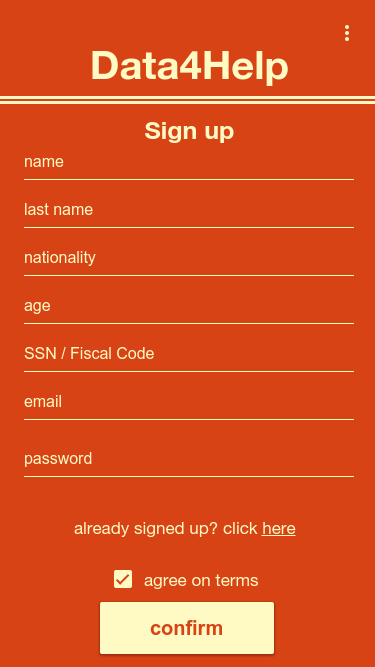
\includegraphics[width=.9\linewidth, height = 7cm, keepaspectratio]{./Images/Mockups/Data4Help/D4HU/D4HU_SignUp.png}
  \caption{Data4Help - User - Sign Up}
\end{subfigure}%
\begin{subfigure}{.33\textwidth}
  \centering
  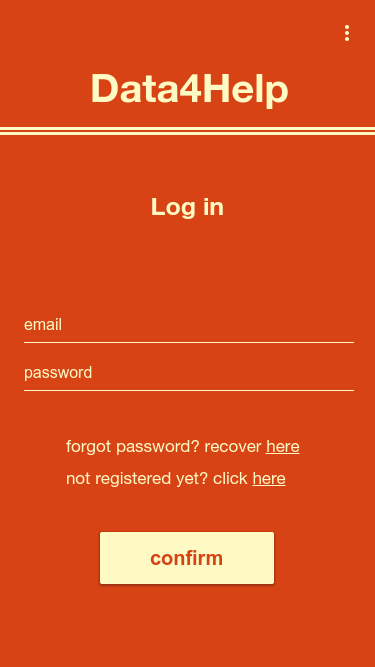
\includegraphics[width = .9\linewidth, height = 7cm, keepaspectratio]{./Images/Mockups/Data4Help/D4HU/D4HU_Login.png}
  \caption{Data4Help - User - Login}
\end{subfigure}
\begin{subfigure}{.33\textwidth}
  \centering
  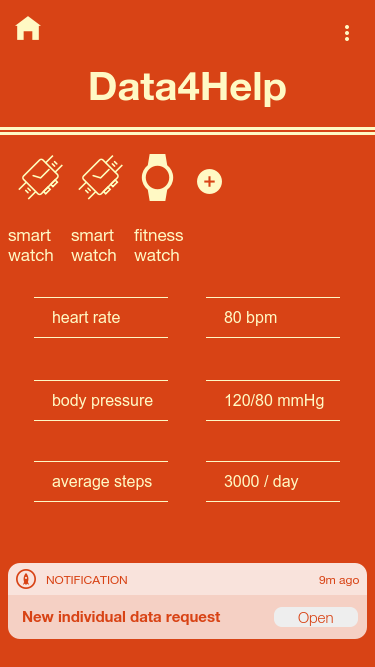
\includegraphics[width = .9\linewidth, height = 7cm, keepaspectratio]{./Images/Mockups/Data4Help/D4HU/D4HU_Homepage.png}
  \caption{Data4Help - User - Homepage}
\end{subfigure}
\end{figure}

  The Sign Up and Login pages are quite self-explanatory.
  The homepage of Data4Help's users consists in a list of the values registered by the sensors paired with the device and a list of such devices. It's given to the user the possibility to delete and add devices on his account. Moreover, on the bottom of such page is shown a notification panel, whose goal is to tell the user when a third party is willing to access his private information.


\paragraph{D4HTP - Sign up and Login}
\begin{figure}[H]
\centering
\begin{subfigure}{.5\textwidth}
  \centering
  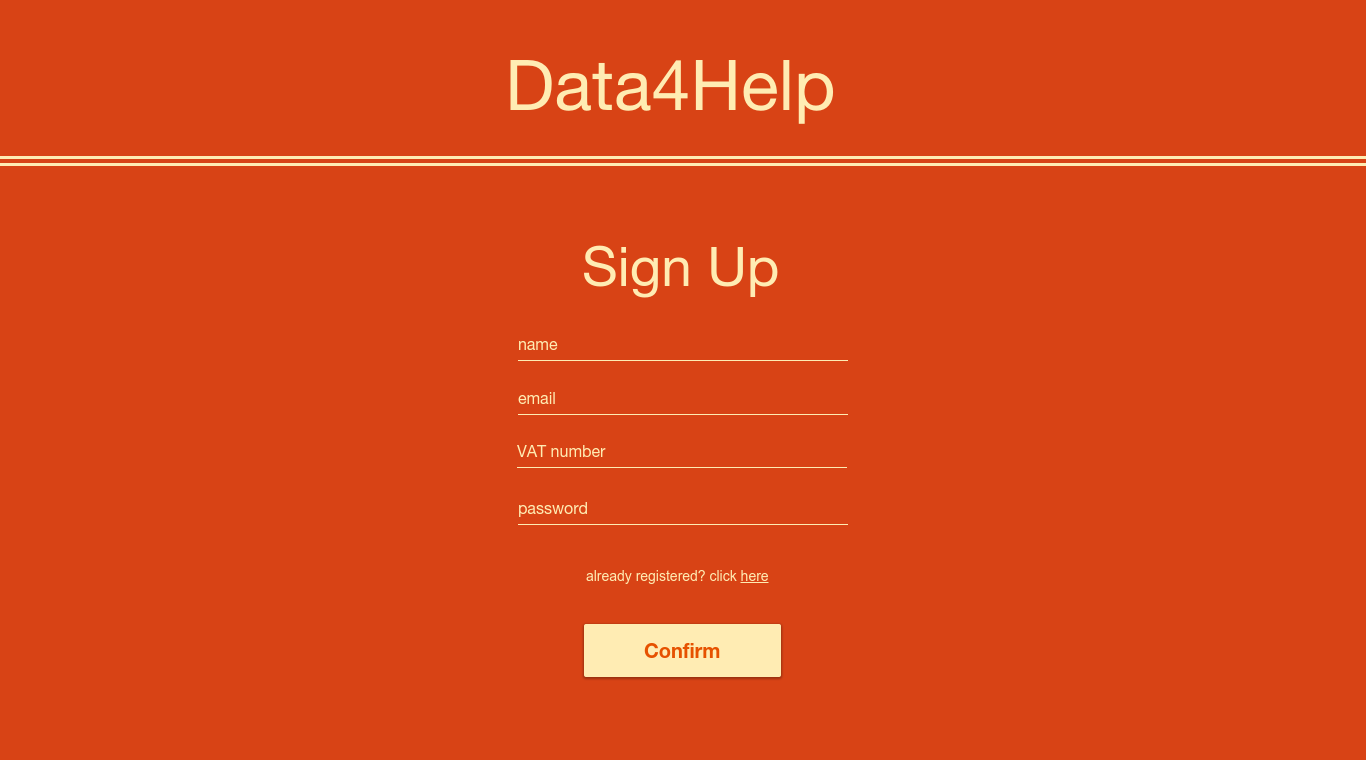
\includegraphics[width=.9\linewidth, height = 7cm, keepaspectratio]{./Images/Mockups/Data4Help/D4HTP/D4HTP_SignUp.png}
  \caption{Data4Help - Third Party - Sign Up}
\end{subfigure}%
\begin{subfigure}{.5\textwidth}
  \centering
  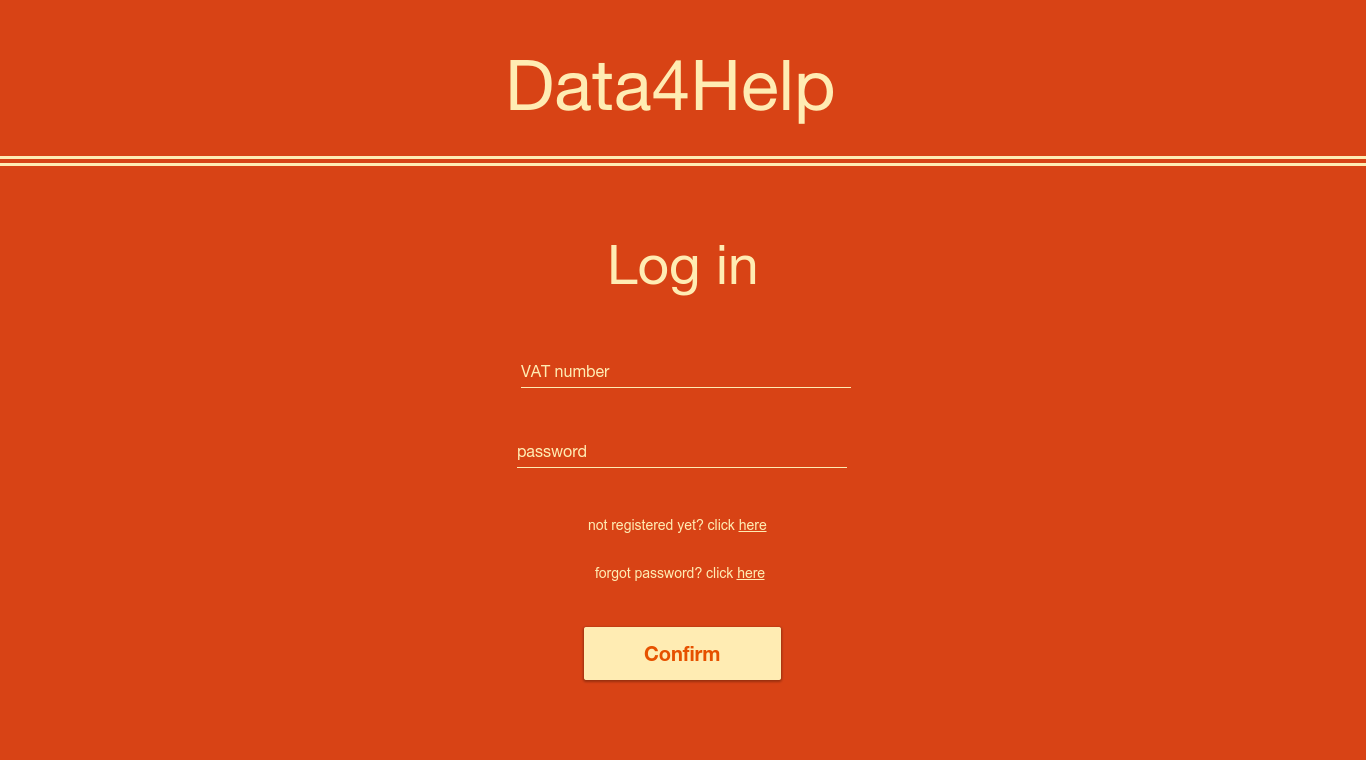
\includegraphics[width = .9\linewidth, height = 7cm, keepaspectratio]{./Images/Mockups/Data4Help/D4HTP/D4HTP_Login.png}
  \caption{Data4Help - Third Party - Login}
\end{subfigure}
\end{figure}
The sign up and login pages of the third parties' version of Data4Help are quite minimalistic. 
Both pages just require the VAT number of the third party and the password. Moreover is offered the chance to switch from login to sign up and viceversa by clicking the underlined text below the password field. 



\paragraph{D4HTP - Homepage}
\begin{figure}[H]
    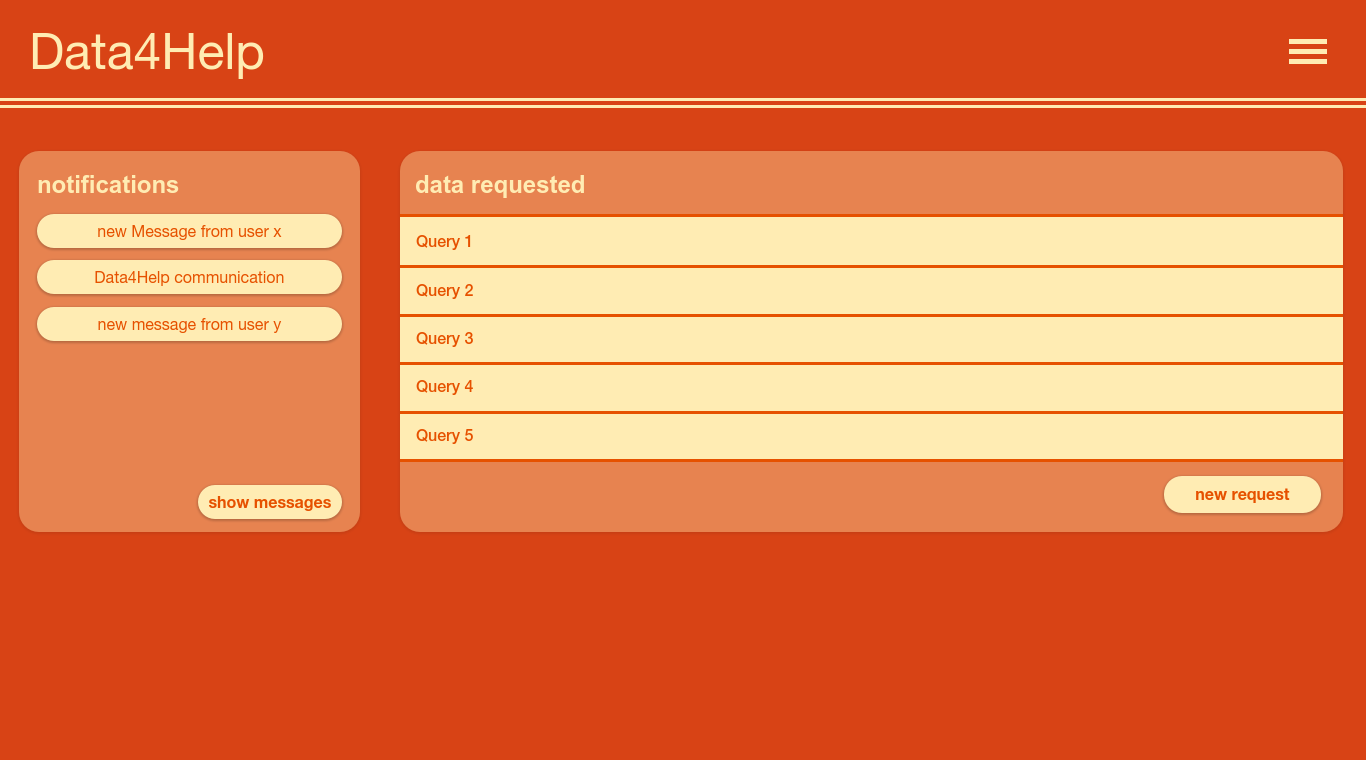
\includegraphics[width=.6\linewidth, height = 20cm, keepaspectratio]{./Images/Mockups/Data4Help/D4HTP/D4HTP_HomePage.png}
    \centering
    \caption{Data4Help - Third Party - Homepage}
    \label{fig:sab}
  \end{figure}
Once the user logged in, he is shown on the left the last notifications (later called "messages") he received. A notification/message is any of the following events:
\begin{itemize}
		\item Information about new versions of the application.
		\item Personal message from Data4Help team's to the third party for any reason (i.e. : communicating the impossibility of satisfying a request)
    \item Query results' detailed information
\end{itemize}
Clicking the "show messages" button, the "messages" page gets opened. 
On the right is displayed the list of requests done by the TP to D4H.
Clcking on any of them a file containing the results of the request gets downloaded.
Clicking on the "new request" button a "new request" page gets opened.




\paragraph{D4HTP - Messages}
\begin{figure}[H]
    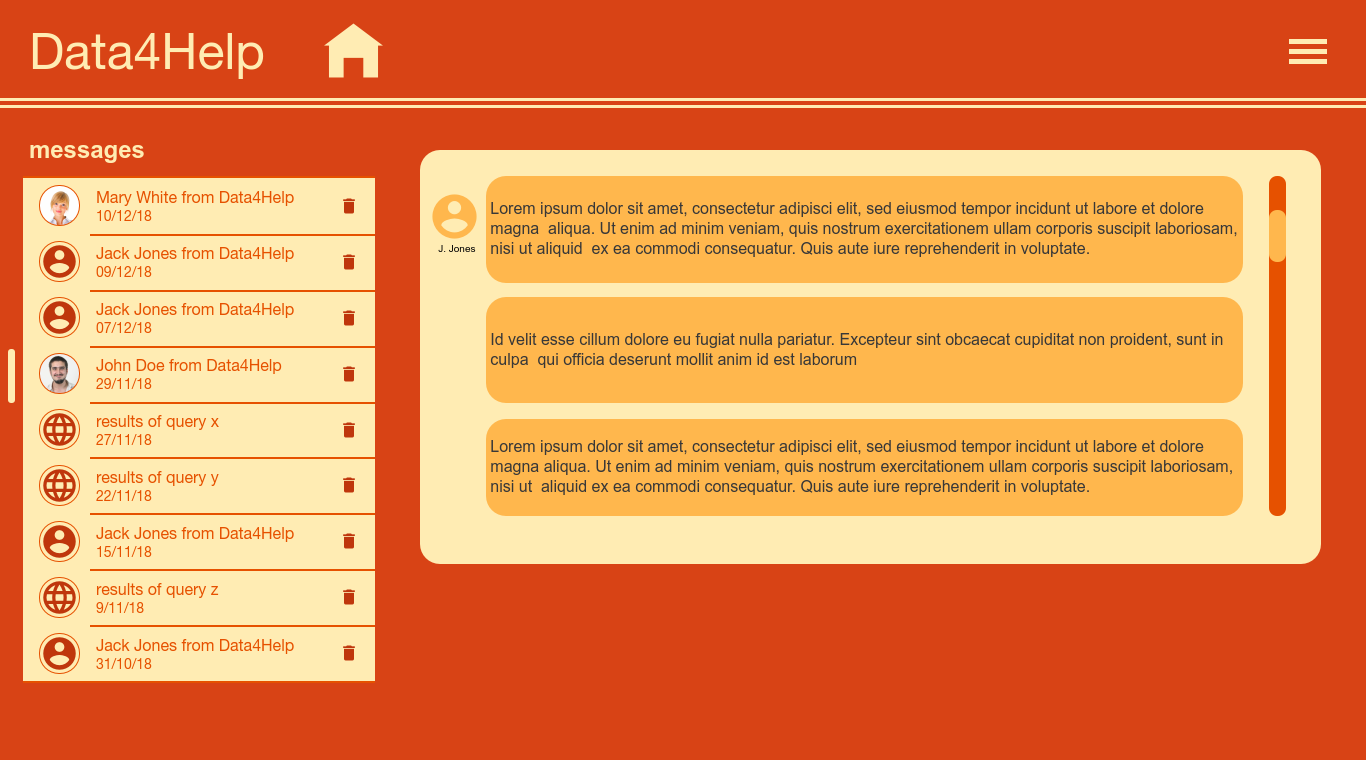
\includegraphics[width=.6\linewidth, height = 20cm, keepaspectratio]{./Images/Mockups/Data4Help/D4HTP/D4HTP_ShowMessages.png}
    \centering
    \caption{Data4Help - Third Party - Messages}
    \label{fig:sab}
  \end{figure}
On the left are shown the messages sent by the Data4Help staff to the TP. 
Once one of such messages gets clicked, the actual message gets shown on the right and a rounded shape appears on the left of the message opened in order to clearly show which message has been opened.

\begin{figure}[H]
    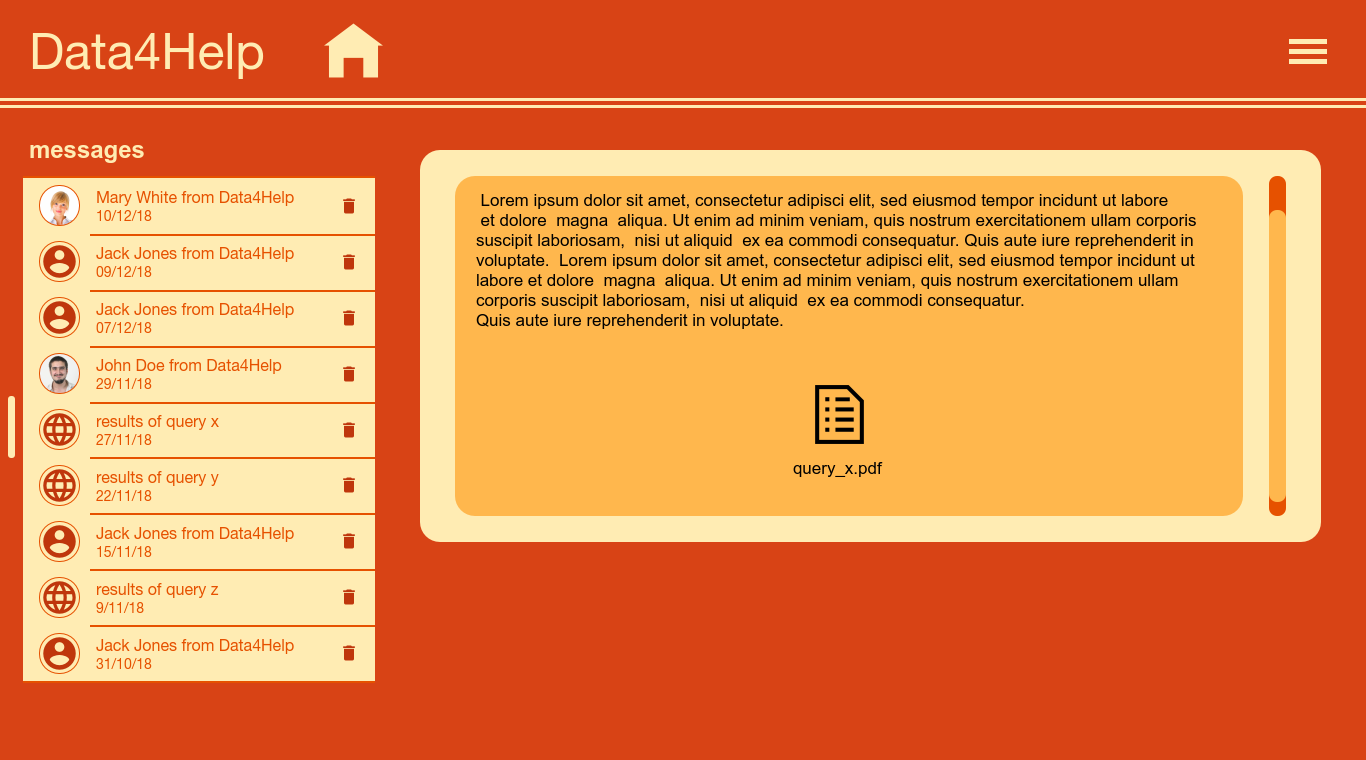
\includegraphics[width=.6\linewidth, height = 20cm, keepaspectratio]{./Images/Mockups/Data4Help/D4HTP/D4HTP_ShowQuery.png}
    \centering
    \caption{Data4Help - Third Party - Messages - Query Result}
    \label{fig:sab}
  \end{figure}
Queries results gets shown firstly in such page, as normal messages from Data4Help that contains the following data:
\begin{itemize}
\item A written summary of the request
\item The day the request was made
\item The number of users whose data have been usedT
\item the document itself that contains the result of the query
\end{itemize}
As explicated in the homepage paragraph, such results gets displayed even in the homepage, the fact that they are shown in the messages section as well is a way of returning more information about the query, not merely the data file.
Moreover the home symbol obviously redirects to the homepage.




\paragraph{D4HTP - New Request, Anonymous Aggregated Data, User's Personal Data}
\begin{figure}[H]
    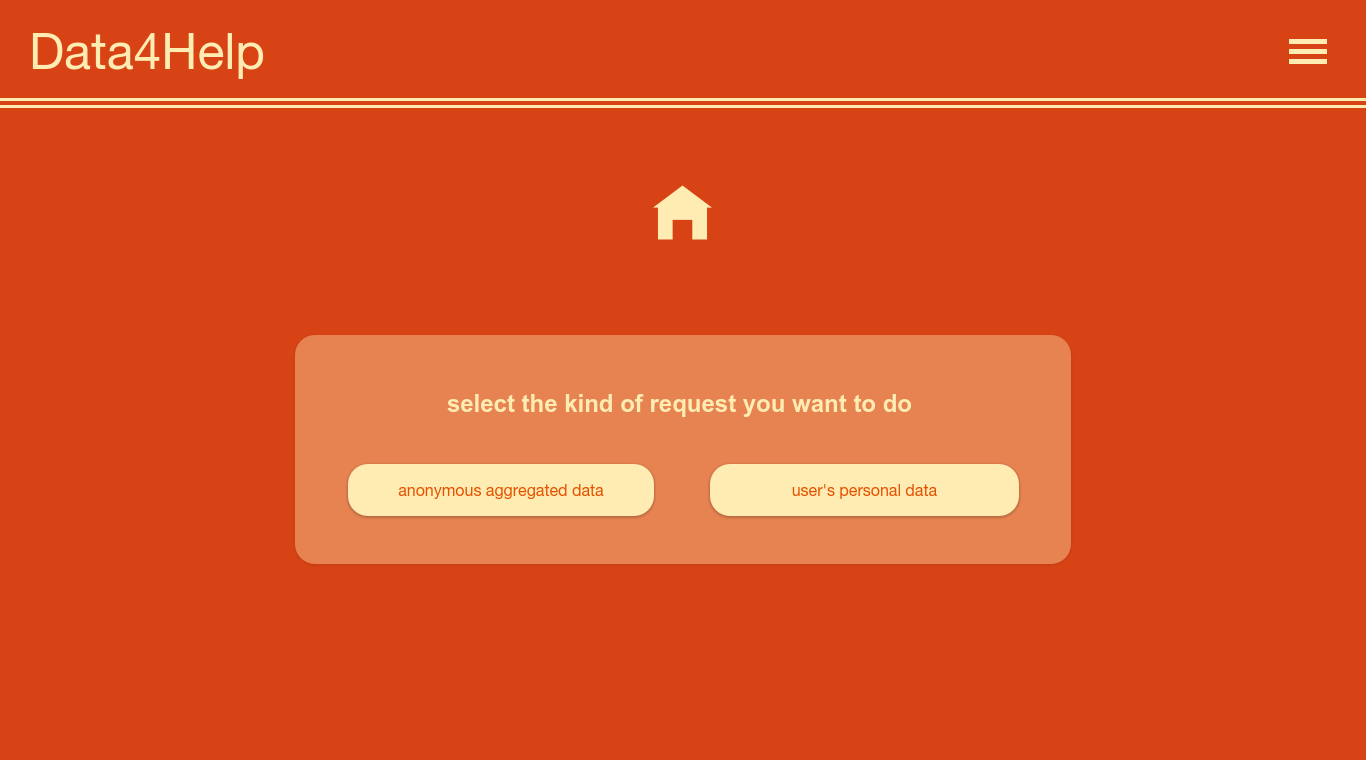
\includegraphics[width=.6\linewidth, height = 20cm, keepaspectratio]{./Images/Mockups/Data4Help/D4HTP/D4HTP_NewQueryRequest.png}
    \centering
    \caption{Data4Help - Third Party - New Query Request}
    \label{fig:sab}
  \end{figure}

the new request page consists in the selection between one of the two possible queries, their names are self-explanatory. 
By clicking on any of them the TP is redirected to the corresponding page.


\begin{figure}[H]
	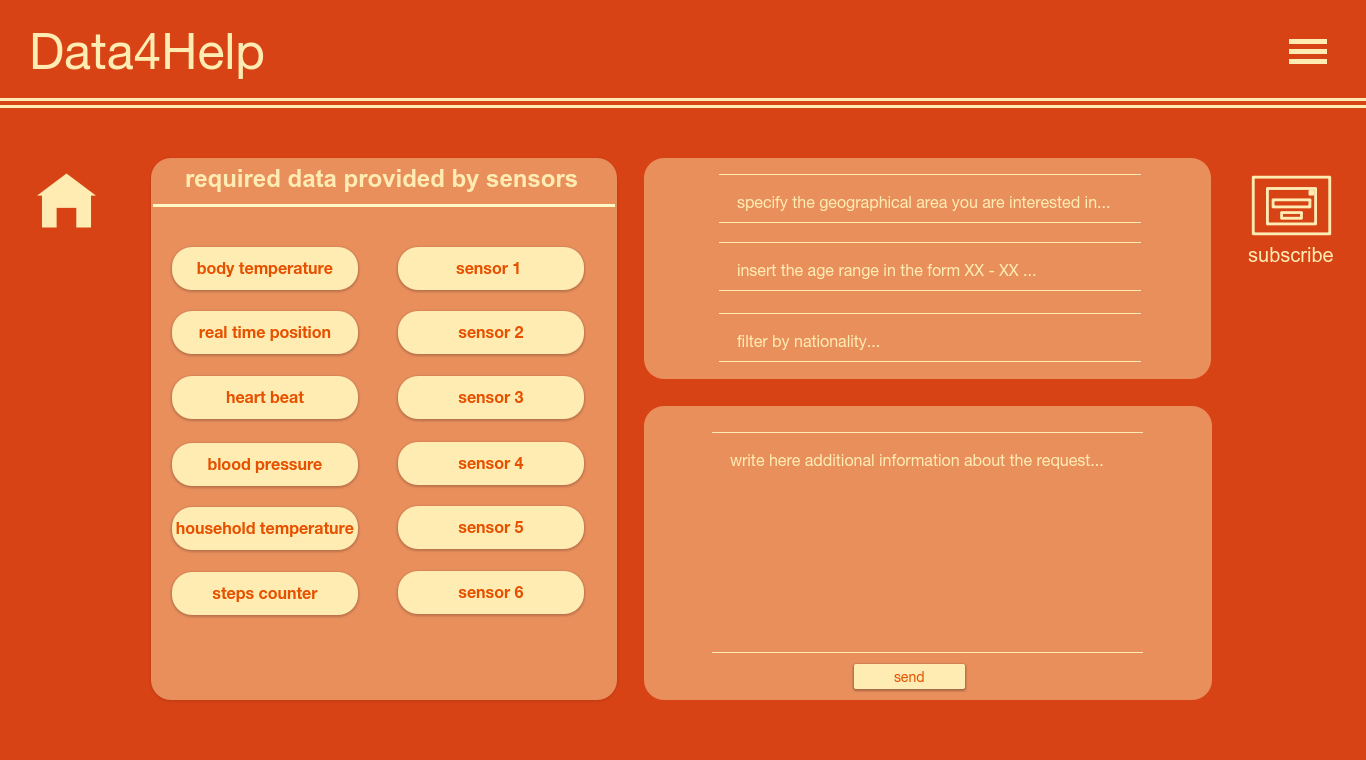
\includegraphics[width=.6\linewidth, height = 20cm, keepaspectratio]{./Images/Mockups/Data4Help/D4HTP/D4HTP_AggregatedDataRequest.png}
	\centering
	\caption{Data4Help - Third Party - Aggregated Data Request}
	\label{fig:sab}
\end{figure}

The Anonymous Aggregated Data page consists in three boxes.
The leftmost one shows all the available sensors from which D4H can get data, the TP will select the ones he is interested in.
Proceeding clockwise the TP is asked what filters he wants to apply to the request (geographical area, age range, and nationality) and in the last box it is asked whether he wants to add any additional information.
By clicking on the "subscribe" button he can subscribe to such request, specifying the period of subscription and the interval of time between one result and the next one.
This latter scene consists in just those two fields. Since it's a simple functionality, it's left to the developer to design it.

\begin{figure}[H]
    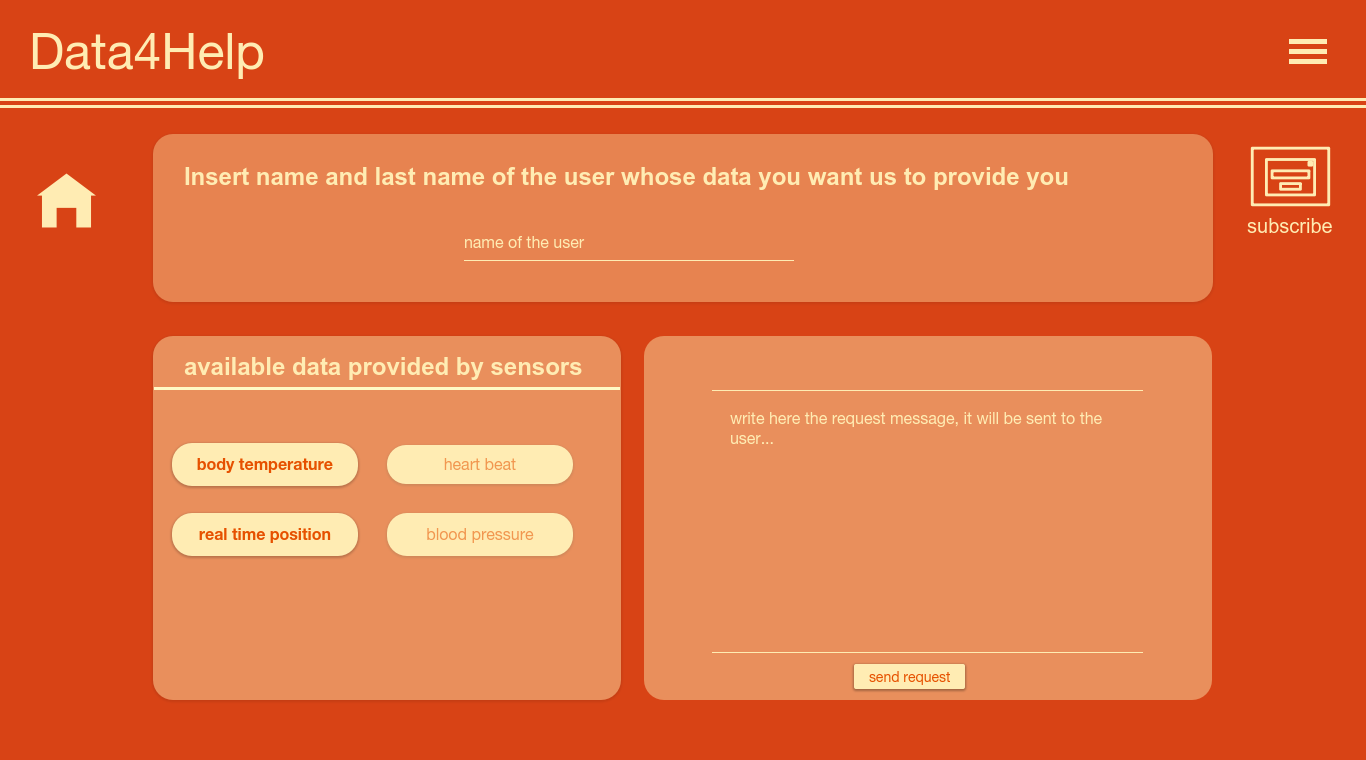
\includegraphics[width=.6\linewidth, height = 20cm, keepaspectratio]{./Images/Mockups/Data4Help/D4HTP/D4HTP_IndividualDataRequest.png}
    \centering
    \caption{Data4Help - Third Party - Individual Data Request}
    \label{fig:sab}
 \end{figure}
The User's Personal Data page is similar to the latter page presented. In the "available data provided by sensors" box are shown 4 sensors, the TP can select any of such sensors to be provided to him.
The subscribe button works as described earlier. 

\paragraph{ASOS - Sign up, Login \& Homepage}
\begin{figure}[H]
\centering
\begin{subfigure}{.33\textwidth}
  \centering
  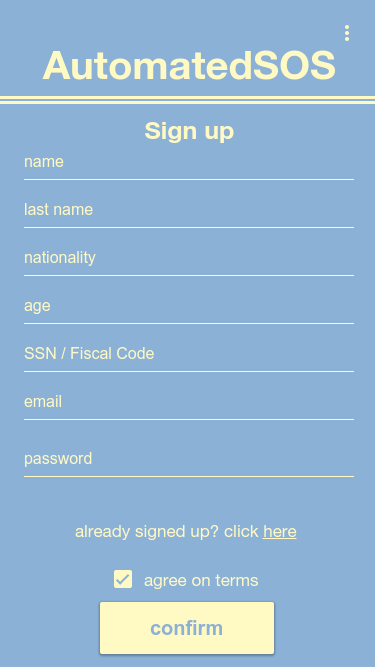
\includegraphics[width=.9\linewidth, height = 7cm, keepaspectratio]{./Images/Mockups/AutomatedSOS/ASOS_SignUp.png}
  \caption{AutomatedSOS - Sign Up}
\end{subfigure}%
\begin{subfigure}{.33\textwidth}
  \centering
  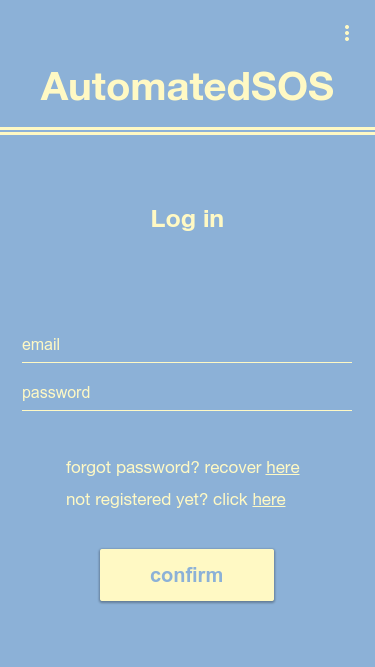
\includegraphics[width = .9\linewidth, height = 7cm, keepaspectratio]{./Images/Mockups/AutomatedSOS/ASOS_Login.png}
  \caption{AutomatedSOS - Login}
\end{subfigure}
\begin{subfigure}{.33\textwidth}
  \centering
  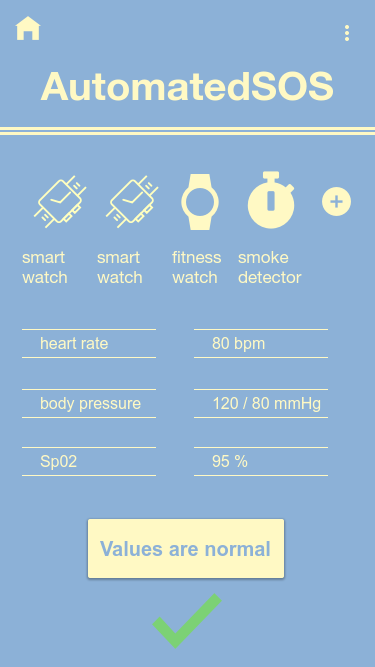
\includegraphics[width = .9\linewidth, height = 7cm, keepaspectratio]{./Images/Mockups/AutomatedSOS/ASOS_Homepage.png}
  \caption{AutomatedSOS - Homepage}
\end{subfigure}
\end{figure}

  Such mockups are very similar to the ones shown for the users version of Data4Help, the only difference is in the homepage mockup, where the notification panel has been substituted with a text that tells the user whether its values are normals or not, in the latter case the user is told whether the ambulance has been called.



  \paragraph{T4R - Sign up, Login \& Homepage}
\begin{figure}[H]
\centering
\begin{subfigure}{.33\textwidth}
  \centering
  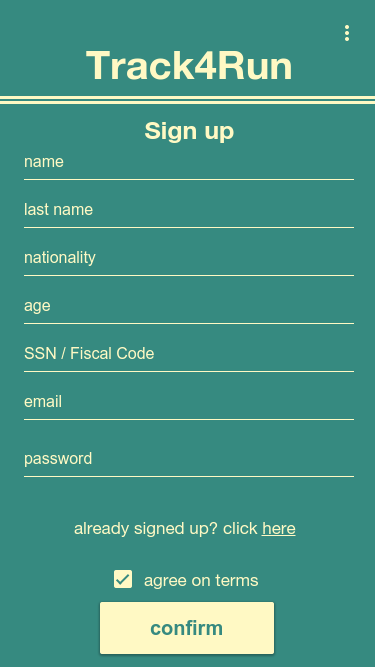
\includegraphics[width=.9\linewidth, height = 7cm, keepaspectratio]{./Images/Mockups/Track4Run/T4R_SignUp.png}
  \caption{Track4Run - Sign Up}
\end{subfigure}%
\begin{subfigure}{.33\textwidth}
  \centering
  \includegraphics[width = .9\linewidth, height = 7cm, keepaspectratio]{./Images/Mockups/Track4Run/T4R_Login.png}
  \caption{Track4Run - Login}
\end{subfigure}
\begin{subfigure}{.33\textwidth}
  \centering
  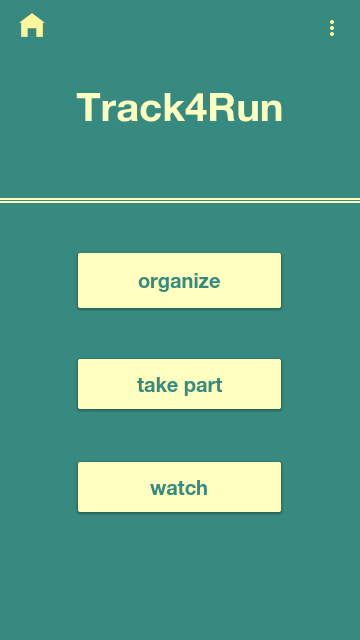
\includegraphics[width = .9\linewidth, height = 7cm, keepaspectratio]{./Images/Mockups/Track4Run/T4R_Homepage.png}
  \caption{Track4Run - Homepage}
\end{subfigure}
\end{figure}
  The homepage of Track4Run gives the user the chance of choosing between three possible actions to be performed.



   \paragraph{T4R - Organize}
\begin{figure}[H]
\centering
\begin{subfigure}{.5\textwidth}
\centering
    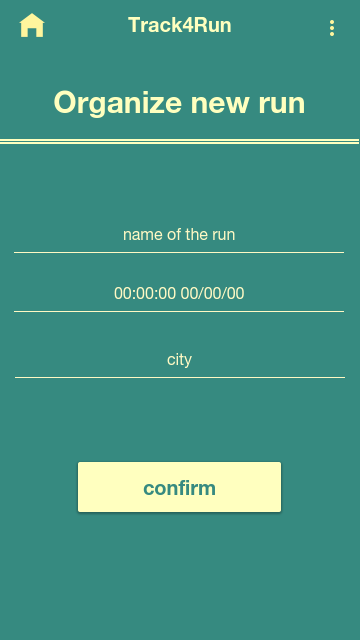
\includegraphics[width=.9\linewidth, height = 7cm, keepaspectratio]{./Images/Mockups/Track4Run/T4R_Organize.png}    
    \caption{Track4Run - Organize}
  \end{subfigure}%
\begin{subfigure}{.5\textwidth}
\centering
    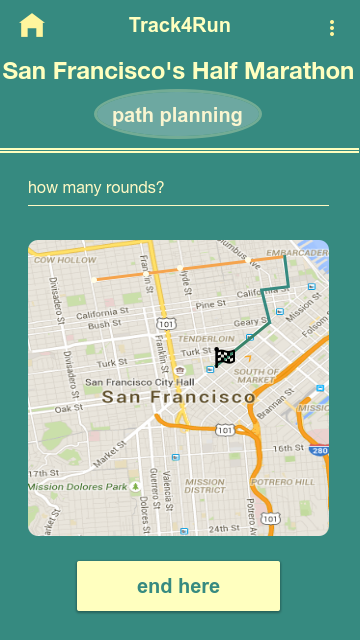
\includegraphics[width=.9\linewidth, height = 7cm, keepaspectratio]{./Images/Mockups/Track4Run/T4R_Organize_SetPath.png}
    \caption{Track4Run - Organize - Set Path}
  \end{subfigure}
\end{figure}

  When the user chooses to organize a run, he is first brought to a page in which he gets asked to fill a form with the name of such run, the date and hour of its occurrence and the city where it will be held. After clicking on the "confirm" button he gets asked to draw the path. A possible solution for such interaction is shown in the figure "Track4Run - Organize - Set Path": the user selects one out of a number of possible nodes (intersections) in the city he has selected and afterwards he clicks on the intersection where he wants to change direction or to end the run. In the second case, after having clicked on the second node he would click on the "end here" button. In the mockup the nodes are displayed in yellow, the street which is getting chosen in orange and the path temporarily selected in water green.




\paragraph{T4R - Take Part}
\begin{figure}[H]
\centering
\begin{subfigure}{.5\textwidth}
    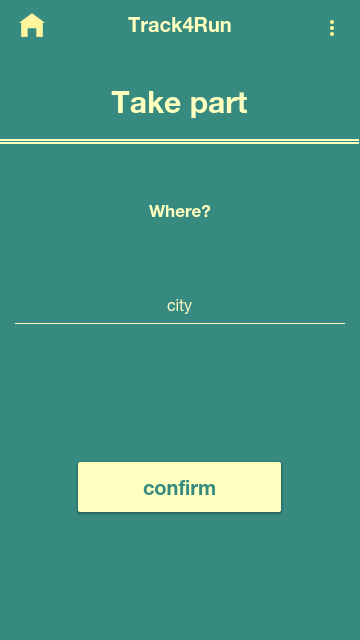
\includegraphics[width=.9\linewidth, height = 7cm, keepaspectratio]{./Images/Mockups/Track4Run/T4R_TakePart1.png}
    \centering
    \caption{Track4Run - Take Part - Step 1}
  \end{subfigure}%
\begin{subfigure}{.5\textwidth}
    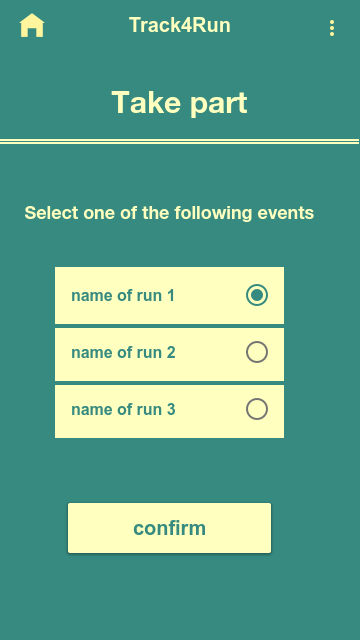
\includegraphics[width=.9\linewidth, height = 7cm, keepaspectratio]{./Images/Mockups/Track4Run/T4R_TakePart2.png}
    \centering
    \caption{Track4Run - Take Part - Step 2}
  \end{subfigure}
\end{figure}
  Mockups of the pages displayed after the clicking of the "Take Part" button in the homepage.



\paragraph{T4R - Watch}
\begin{figure}[H]
\centering
\begin{subfigure}{.5\textwidth}
    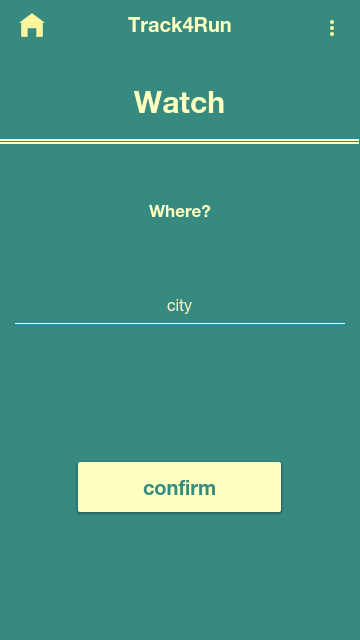
\includegraphics[width=.9\linewidth, height = 7cm, keepaspectratio]{./Images/Mockups/Track4Run/T4R_Watch.png}
    \centering
    \caption{Track4Run - Watch}
  \end{subfigure}%
\begin{subfigure}{.5\textwidth}
    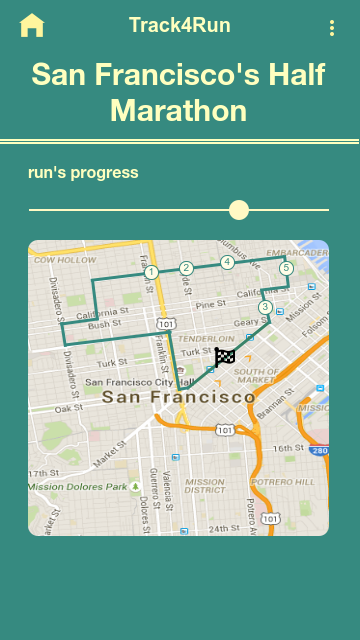
\includegraphics[width=.9\linewidth, height = 7cm, keepaspectratio]{./Images/Mockups/Track4Run/T4R_Watch_Map.png}
    \centering
    \caption{Track4Run - Watch - Map}
  \end{subfigure}
\end{figure}
  Mockups of the pages displayed after the clicking of the "Watch" button.
  the figure (b) represents a live run: the circles within the path represent the partecipants, identified by an id number, which is supposedly given to them in the moment of the registration to the run. The flag represents the starting point, and the orange arrows aside of the path represent the direction of travel.
  \newline
  Any omitted detail is left to the developer to be thought. The mockups presented offer just a guideline for the development of the user interface.








%%
\newpage
{\color{secblue}\subsection{User Experience Diagrams}}
The following diagrams have been written in order to offer a better understanding of the interaction between the users and the applications. 
It is suggested to look to such diagrams while reading the description of the corresponding mockups.
It is not explicitly shown in the diagrams, but from any page it's possible to go to the homepage of the developed apps.

\begin{figure}[H]
    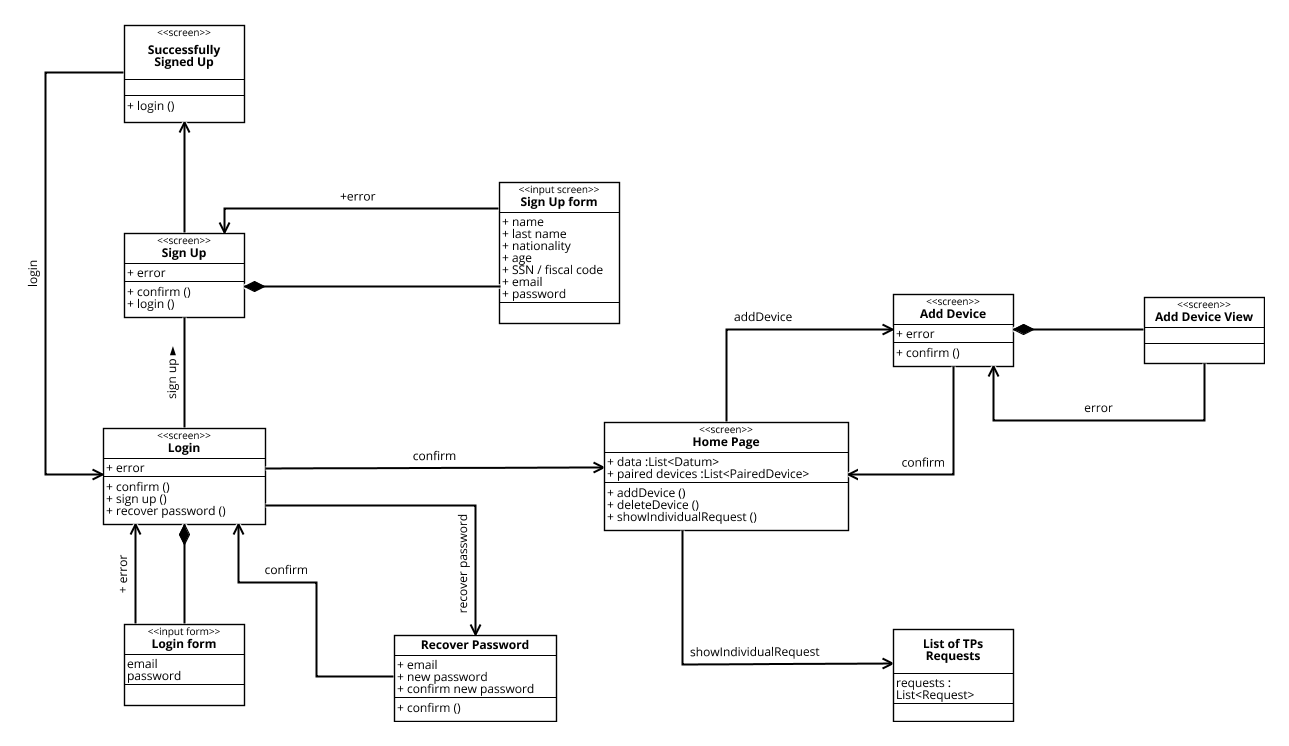
\includegraphics[width=\linewidth, height = 20cm, keepaspectratio]{./Images/DD_UXD_D4H_U.png}
    \centering
    \caption{UX Diagram - Data4Help - User}
    \label{fig:sab}
 \end{figure}

 \begin{figure}[H]
    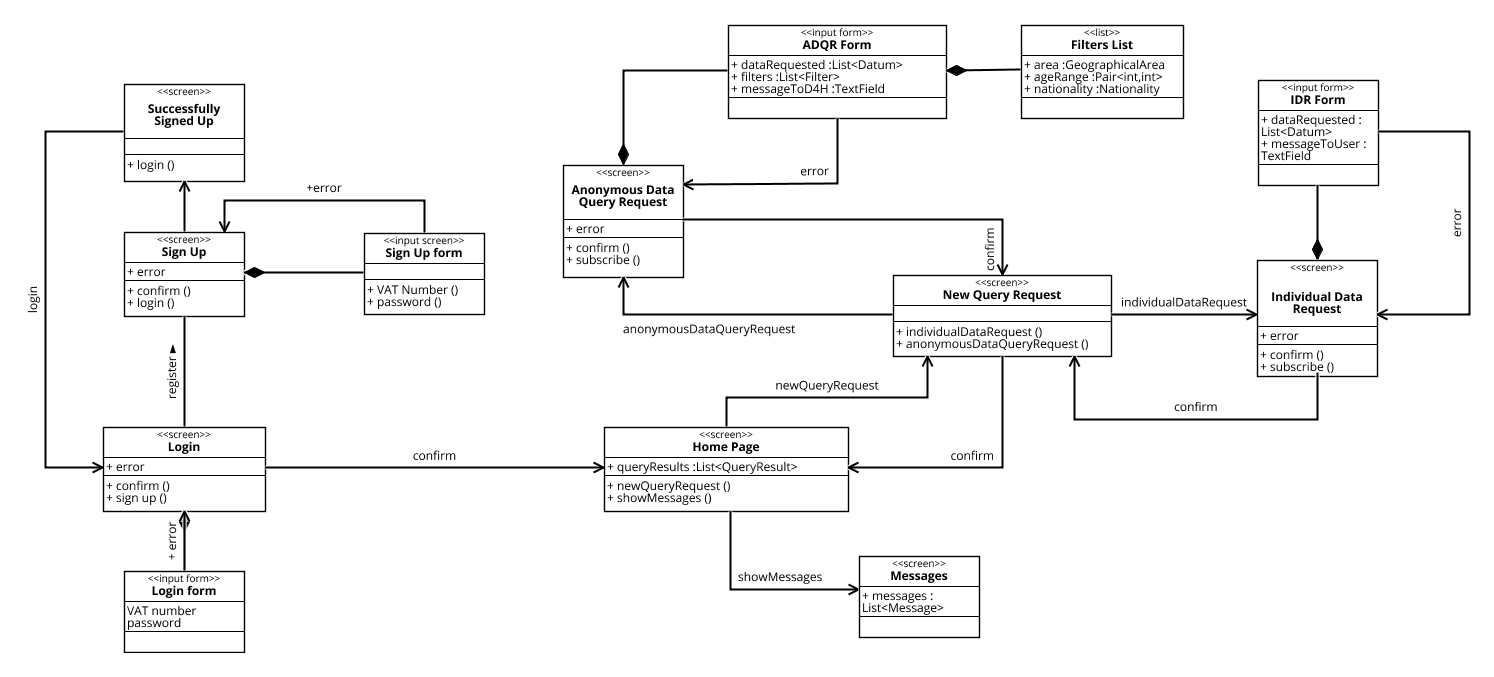
\includegraphics[width=\linewidth, height = 20cm, keepaspectratio]{./Images/DD_UXD_D4H_TP.png}
    \centering
    \caption{UX Diagram - Data4Help - Third Party}
    \label{fig:sab}
 \end{figure}

 \begin{figure}[H]
    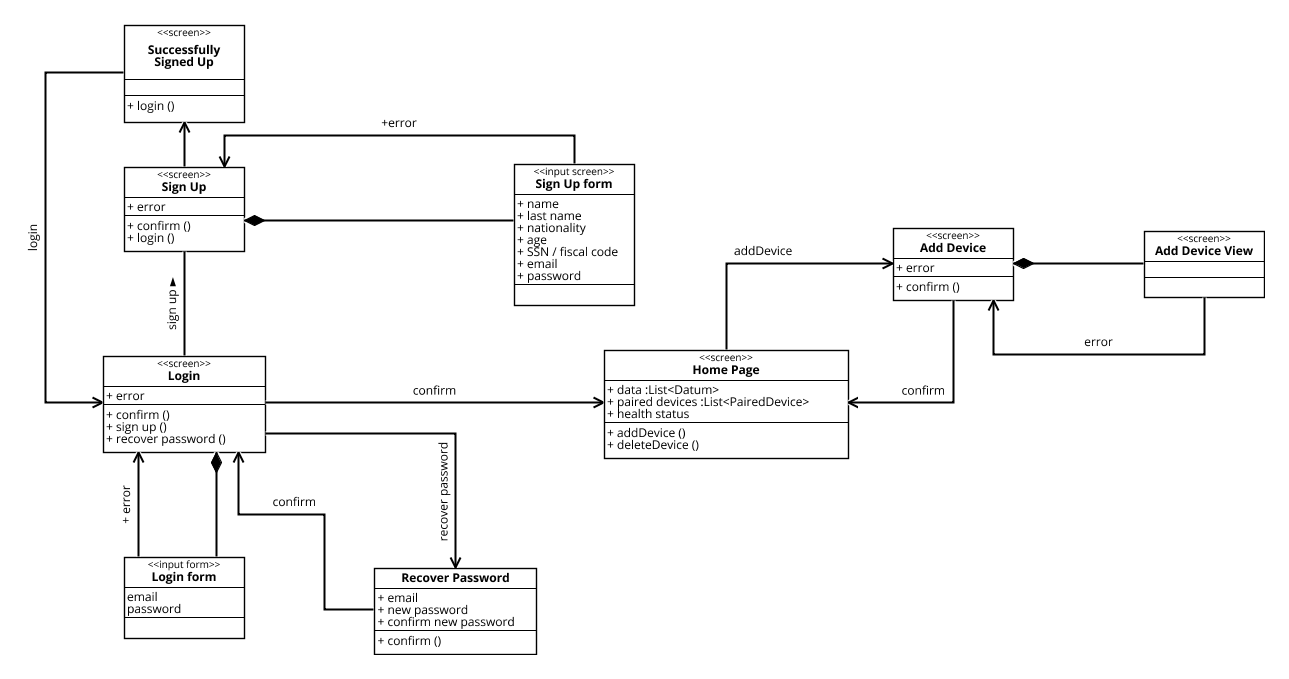
\includegraphics[width=\linewidth, height = 20cm, keepaspectratio]{./Images/DD_UXD_ASOS.png}
    \centering
    \caption{UX Diagram - AutomatedSOS - User}
    \label{fig:sab}
 \end{figure}

 \begin{figure}[H]
    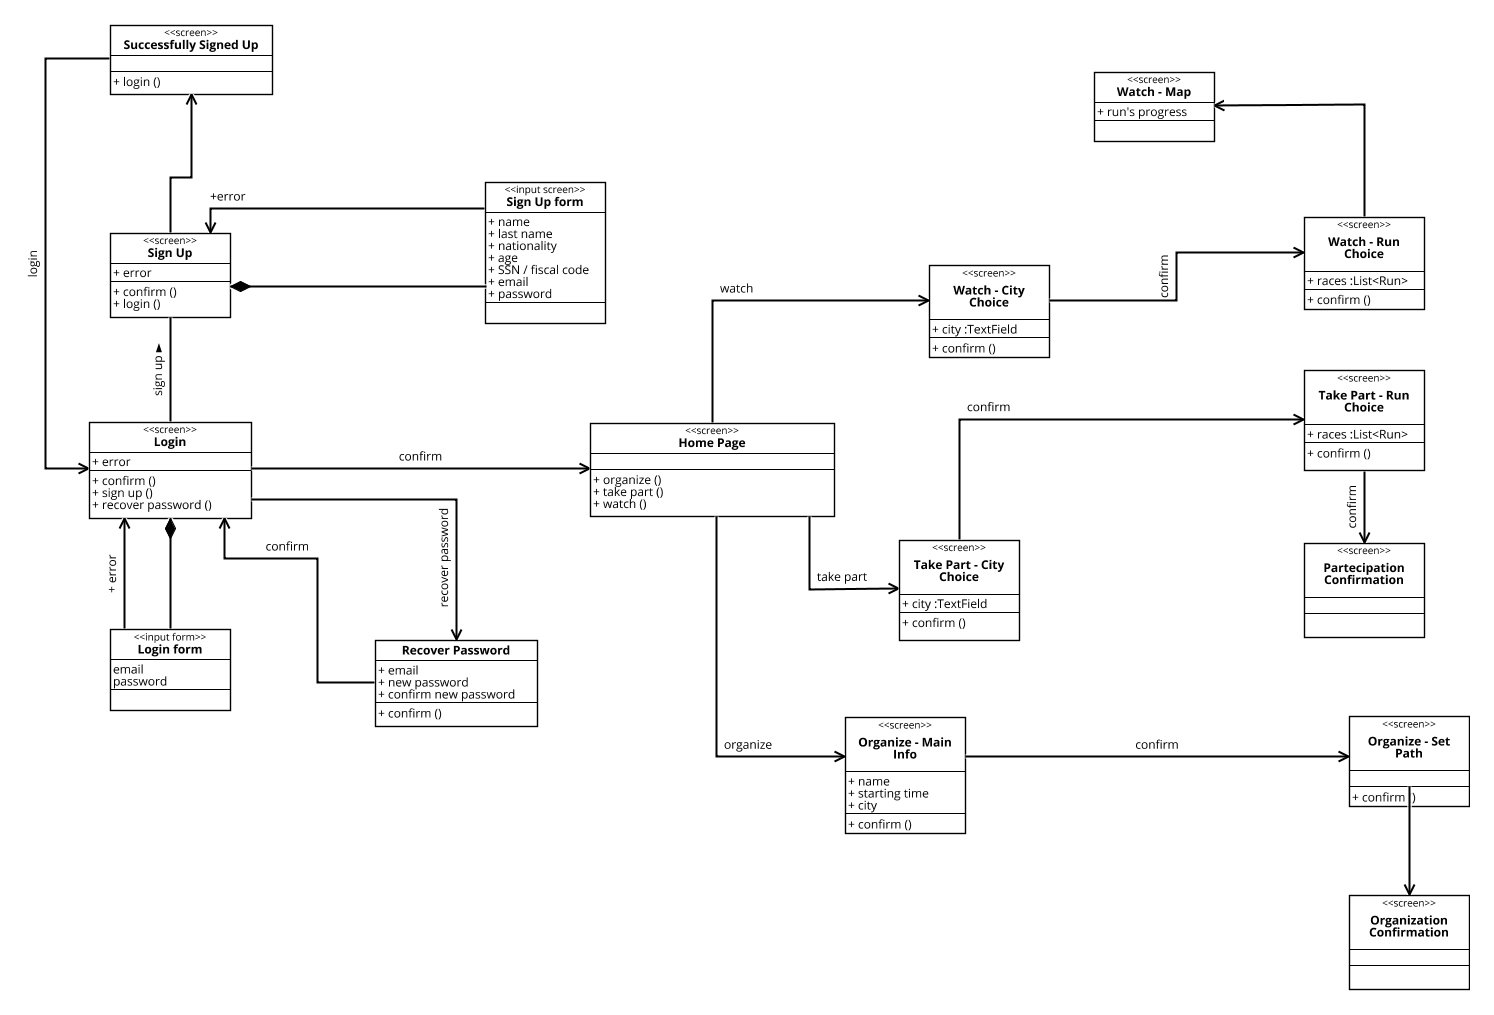
\includegraphics[width=\linewidth, height = 20cm, keepaspectratio]{./Images/DD_UXD_T4R.png}
    \centering
    \caption{UX Diagram - Track4Run - User}
    \label{fig:sab}
 \end{figure}

